\documentclass[mathserif,serif]{beamer}
\useoutertheme{infolines}
%\usepackage{tabularx}
%\usepackage{amsmath}

\title[Oral Presentation]{Search for chargino and neutralino production in final states with two same-sign leptons, jets and missing transverse momentum at $\sqrt{s} = 13$ TeV with the ATLAS detector}
\author[]
{
Samuel Lo \inst{1}
}
\institute[]
{
\inst{1}
The University of Hong Kong
}
\date[]{\today}

\newcommand\Wider[2][2em]{%
\makebox[\linewidth][c]{%
\begin{minipage}{\dimexpr\textwidth+#1\relax}
\raggedright
\centering#2
\end{minipage}%
}%
}

\begin{document}

\frame{\titlepage}
\frame{\tableofcontents}

\section{Introduction}
\begin{frame}
\begin{center}
\huge
Introduction
\end{center}
\end{frame}

\begin{frame}{Standard Model : Fundamental Particles}
\begin{itemize}
\item Standard Model(SM) is the current mainstream theory to describe the electromagnetic force, weak force and strong force.
\end{itemize}

\begin{figure}
\centering
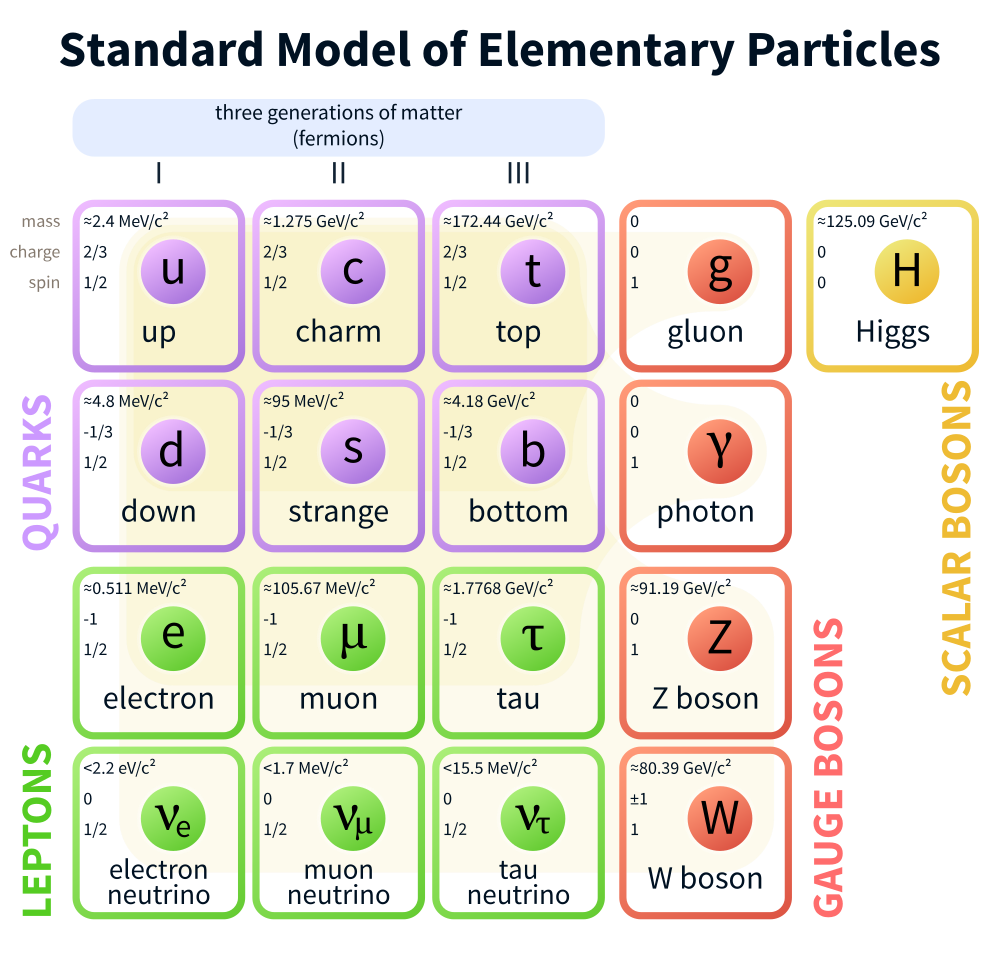
\includegraphics[width=0.5\textwidth]{data/photo/theory/SM_particles.png}
\caption{The ``periodic'' table for all fundamental particles in SM.}
\end{figure}
\end{frame}

\begin{frame}{Standard Model : Fundamental Interaction}
\begin{columns}

\begin{column}{0.5\textwidth}
\begin{figure}
\centering
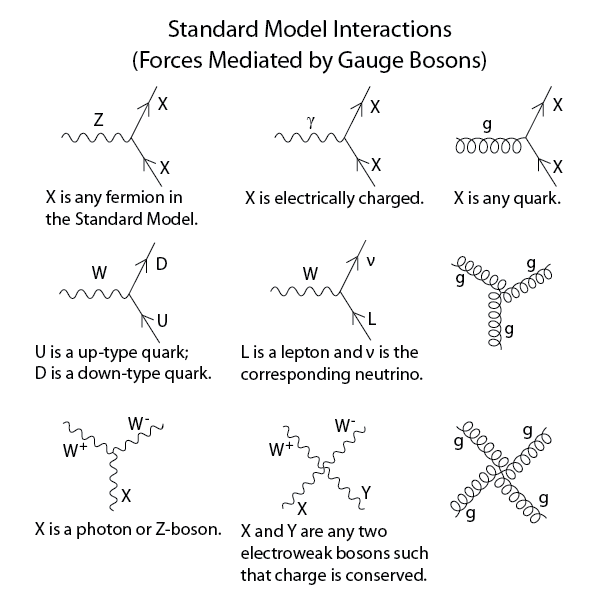
\includegraphics[width=\textwidth]{data/photo/theory/vertices_SM.png}
\caption{All allowed fundamental Feynman vertices in SM, except higgs-related vertices.}
\end{figure}

\end{column}

\begin{column}{0.5\textwidth}
\begin{figure}
\centering
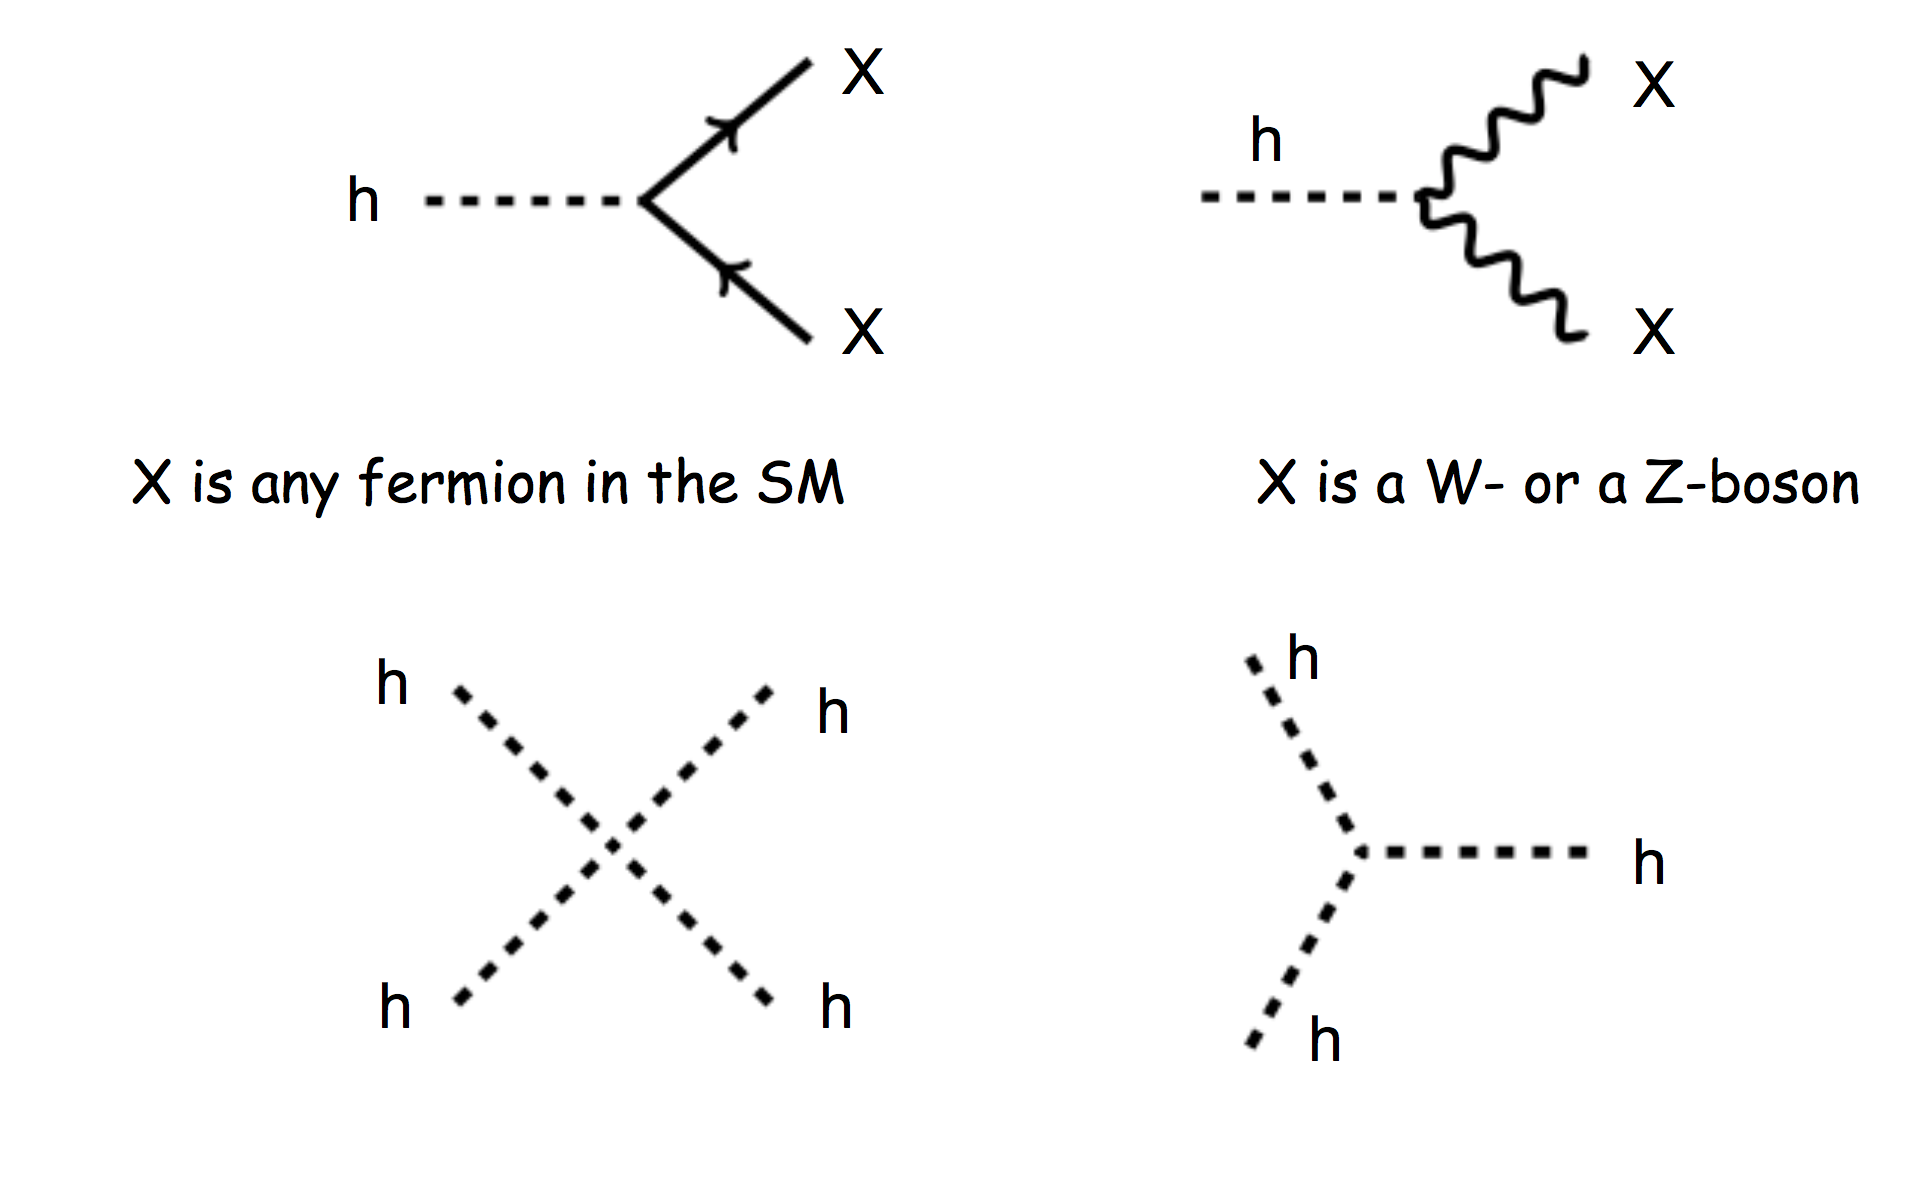
\includegraphics[width=\textwidth]{data/photo/theory/vertices_higgs.png}
\caption{All allowed fundamental higgs-related Feynman vertices in SM.}
\end{figure}
\end{column}

\end{columns}
\end{frame}

\begin{frame}{Standard Model : Limitation}
\begin{itemize}
\item SM cannot explain gravity.
\item SM cannot explain the nature of dark matter.
\item The hierarchy problem
\begin{itemize}
\item Why the weak force is stronger than the gravity by $10^{24}$.
\item Why the Higgs mass is much lighter than the Planck mass.
\item At very high energy scale, the Higgs boson mass is strongly sensitive to quantum corrections.
\end{itemize}
\end{itemize}
\end{frame}

\begin{frame}{Supersymmetry}
\begin{itemize}
\item Supersymmetry(SUSY) is an extension of the Standard Model.
\item It can solve the hierarchy problem of Higgs mass.
\item It can explain the nature of dark matter.
\end{itemize}
\end{frame}

\begin{frame}{Supersymmetry : MSSM}
\begin{itemize}
\item Minimal Supersymmetric Standard Model(MSSM) is the simplest realization of the supersymmetry.
\item It predicts that each particle in the Standard Model has its own partner particle, called the superpartner.
\item The spin of the superpartner will differ from the Standard Model particle by 1/2.
\item A symmetry between the fermions and bosons.
\end{itemize}
\begin{figure}
\centering
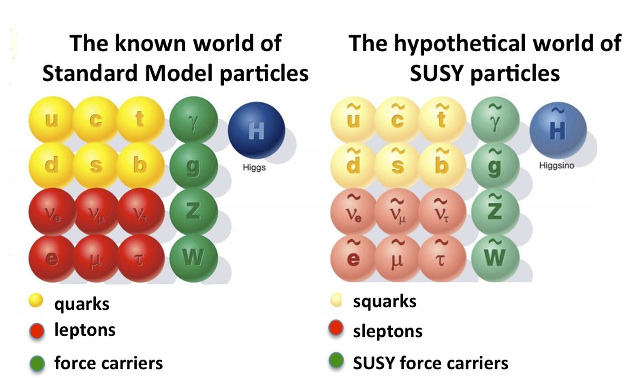
\includegraphics[width=0.4\textwidth]{data/photo/theory/SM-SUSY-diagram.jpg}
\caption{The particles in Standard Model and their corresponding superpartners and their names.}
\end{figure}
\end{frame}

\begin{frame}{Supersymmetry : Superpartners}
\begin{itemize}
\item In the MSSM, one more neutral Higgs filed $H$ and two more charged Higgs fileds $H^+$, $H^-$ needed to be introduced.
\item In SM electro-weak bosons, there are in total 4 neutral bosons: $\gamma$, $Z$, $h$ and $H$, and 4 charged bosons: $W^+$, $W^-$, $H^+$ and $H^-$.
\item The superpartners of the 4 neutral bosons together form 4 mass eigenstates, called neutralinos: $\tilde{\chi}_1^0$, $\tilde{\chi}_2^0$, $\tilde{\chi}_3^0$ and $\tilde{\chi}_4^0$.
\item The superpartners of the 4 charged bosons together form two mass eigenstates with electric charge $\pm 1$, called charginos: $\tilde{\chi}_1^\pm$ and $\tilde{\chi}_2^\pm$.
\end{itemize}

\begin{table}[htbp]
\tiny
\centering
\scalebox{0.8}{
\begin{tabular}{|c|cccc|cccc|}
\hline
\hline
Type & SM particle & Symbol & Spin & R-parity & Superpartner & Symbol & Spin & R-parity \\
\hline
\hline
Fermions & Quark  & $q$ & $\frac{1}{2}$ & +1 & Squark  & $\tilde{q}$ & 0 & -1 \\
& Lepton & $l$ & $\frac{1}{2}$ & +1 & Slepton & $\tilde{l}$ & 0 & -1 \\
\hline
Gluon & Gluon  & $g$ & $1$ & +1 & Gluino & $\tilde{g}$ & $\frac{1}{2}$ & -1  \\
\hline
Neutral EW Bosons & Photon         & $\gamma$ & $1$ & +1
&  &  &  &  \\
& Z Boson        & $Z$      & $1$ & +1
& Neutralinos & $\tilde{\chi}_1^0$, $\tilde{\chi}_2^0$, $\tilde{\chi}_3^0$, $\tilde{\chi}_4^0$ & $\frac{1}{2}$ & -1 \\
& Neutral Higgs  & $h$,$H$  & $0$ & +1
&  &  &  &  \\
\hline
Charged EW Bosons & W Boson        & $W^+$, $W^-$  & $1$ & +1
& Charginos & $\tilde{\chi}_1^\pm$, $\tilde{\chi}_2^\pm$ & $\frac{1}{2}$ & -1 \\
& Charged Higgs  & $H^+$, $H^-$  & $0$ & +1
&  &  &  &  \\
\hline
\hline
\end{tabular}
}
\caption{\scriptsize The spin and R-parity for the Standard Model particles and their superpartners.}
\end{table}

\end{frame}

\begin{frame}{Supersymmetry : R-parity}
\begin{itemize}
\item The baryon number $B$ is defined by $\frac{1}{3} (n_q - n_{\bar{q}})$, where $n_q$ is the number of quarks and $n_{\bar{q}}$ is the number of anti-quarks.
\item The lepton number $L$ is defined by $n_l - n_{\bar{l}}$, where $n_l$ is the number of leptons and $n_{\bar{l}}$ is the number of anti-leptons.
\item In SM, $(B-L)$ is conserved. But in MSSM, it is no longer conserved.
\item To keep $(B-L)$ conservation and prevent the proton decay, the R-parity $P_R$ is introduced.
\begin{equation*}
P_R = (-1)^{3(B-L)-2s}
\end{equation*}
where s is the spin.
\end{itemize}
\end{frame}

\begin{frame}{Supersymmetry : R-parity}
\begin{itemize}
\item All SM particles have R-parity $+1$, while all SUSY particles have R-parity $-1$.
\item If the R-parity is conserved, the lightest supersymmetric particle (LSP) cannot decay and is stable.
\item If the LSP is electrically neutral and interacts with matter only by the weak interaction and gravity, it could be a candidate for dark matter, for example the lightest neutralinos $\tilde{\chi}_1^0$.
\item In this thesis, the R-parity is assumed to be conserved, and the lightest neutralino $\tilde{\chi}_1^0$ is assumed to be the LSP.
\item Due to the conservation of R-parity, the supersymmetric particles can only be pair-produced, and will eventually decay into SM particles and the lightest neutralino $\tilde{\chi}_1^0$ (i.e. LSP).
\end{itemize}
\end{frame}

\begin{frame}{Our Signal Scenario : Motivation}
\begin{itemize}
\item In the recent searches for the squarks ($\tilde{q}$) and gluinos ($\tilde{g}$), the masses of gluinos and the first and second generation squarks are suggested to be larger than 1 TeV, while the masses of the third generation squarks are still allowed to be below 1 TeV.
\item In this case, the direct pair production of $\tilde{\chi}_1^\pm$  and $\tilde{\chi}_2^0$ may be the dominant SUSY production process at the LHC, if the masses of them are below 1 TeV.
\item In this thesis, their masses are assumed to be the same, and denoted by $m_{\tilde{\chi}_1^\pm , \tilde{\chi}_2^0}$.
\end{itemize}
\begin{figure}
\centering
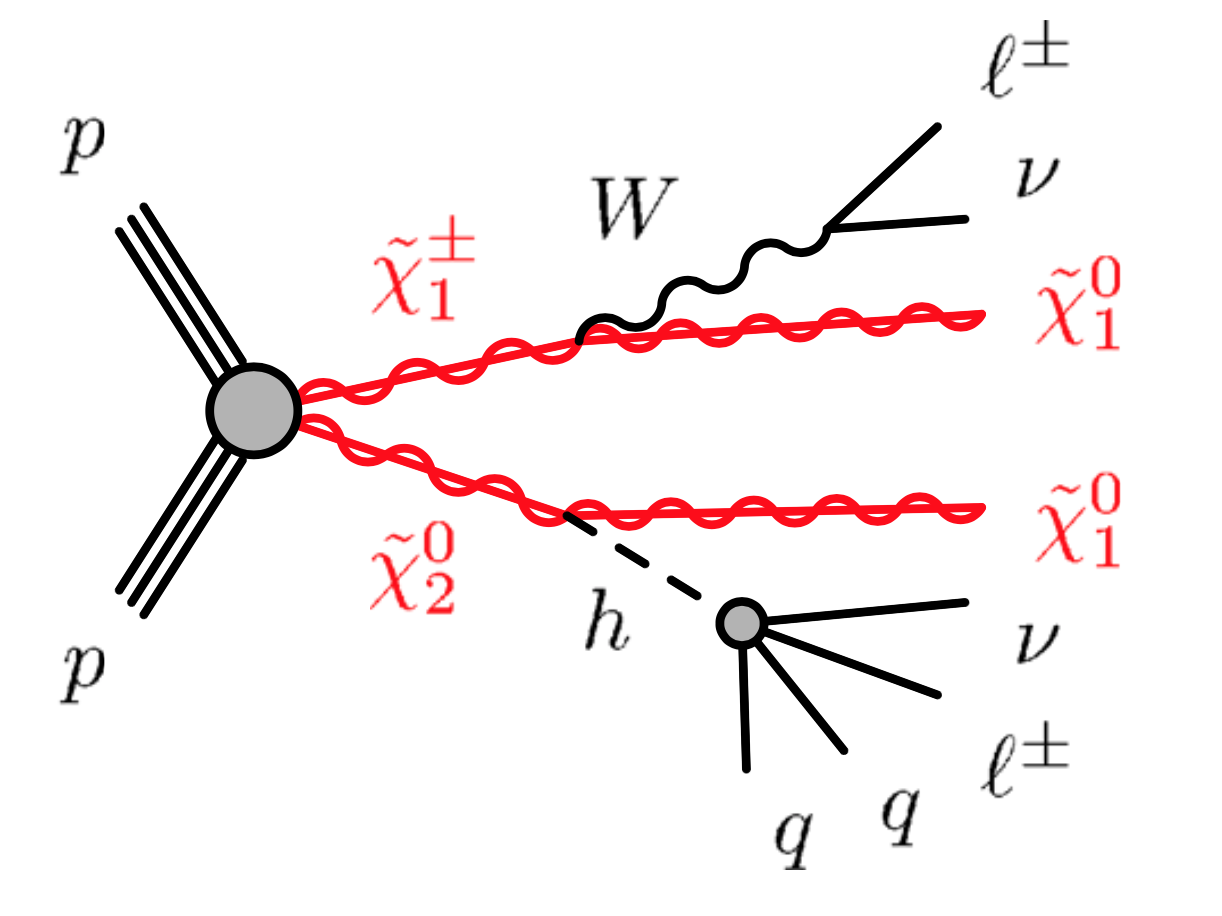
\includegraphics[width=0.3\textwidth]{data/photo/theory/signal_feynman.png}
\end{figure}
\end{frame}

\begin{frame}{Our Signal Scenario : Decay Processes}
\begin{itemize}
\item If all the slepton ($\tilde{l}$) are heavier than $\tilde{\chi}_1^\pm$ and $\tilde{\chi}_2^0$ :
\begin{enumerate}
\item $\tilde{\chi}_1^\pm$ will decay to W boson and $\tilde{\chi}_1^0$ : \\
$\tilde{\chi}_1^\pm \rightarrow W^{\pm} + \tilde{\chi}_1^0$
\item $\tilde{\chi}_2^0$ will decay to the lightest MSSM Higgs boson $h$ and $\tilde{\chi}_1^0$ : \\
$\tilde{\chi}_2^0 \rightarrow h + \tilde{\chi}_1^0$
\end{enumerate}
\end{itemize}
\begin{figure}
\centering
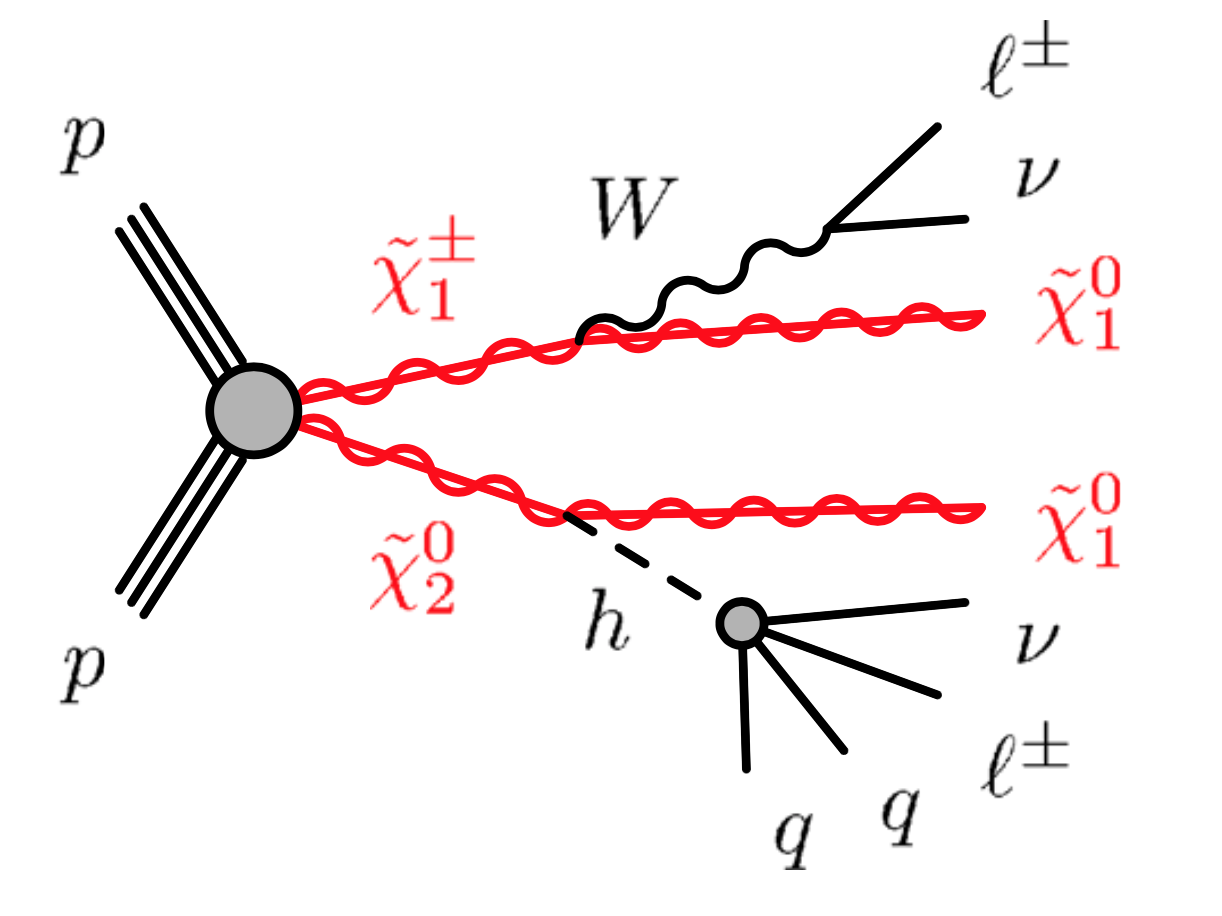
\includegraphics[width=0.3\textwidth]{data/photo/theory/signal_feynman.png}
\caption{The Feynman diagram for our Wh same-sign signal scenario.}
\end{figure}
\end{frame}

\begin{frame}{Our Signal Scenario : Decay Processes}
\begin{itemize}
\item The W boson will further to one lepton (electron or muon) and one neutrino with the SM branching ratio : \\
$W{^\pm} \rightarrow \ell^{\pm} + \nu$
\item The Higgs boson $h$ will eventually decay to one lepton (electron or muon), quarks (i.e. jets) and neutrino(s) by various decay modes with the SM branching ratios. (For example, $h \rightarrow W^{+} W^{-} $ and $h \rightarrow \tau^{+} \tau^{-} $)
\item From now on, a lepton $\ell^{\pm}$ only refer to an electron or muon, but not $\tau$ lepton or neutrino.
\end{itemize}
\begin{figure}
\centering
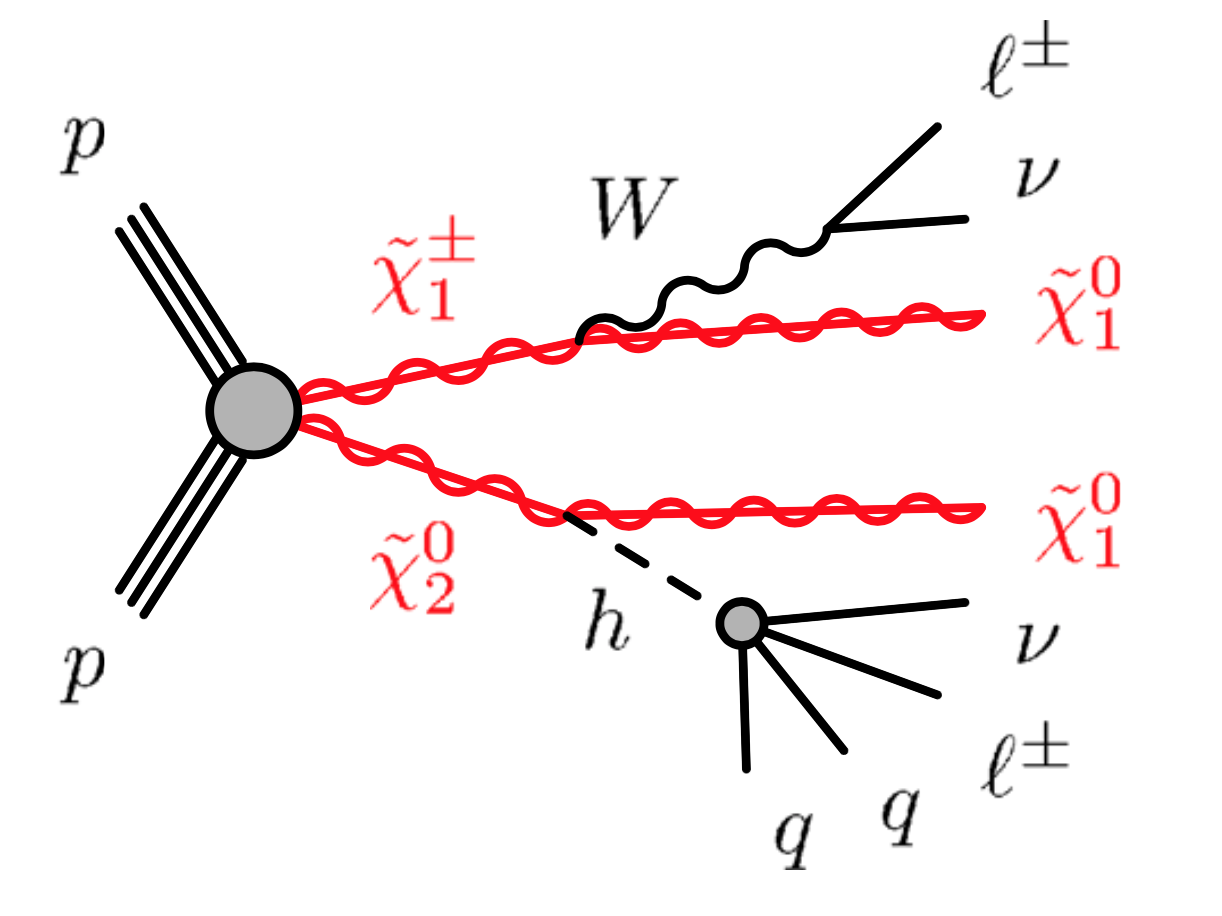
\includegraphics[width=0.3\textwidth]{data/photo/theory/signal_feynman.png}
\end{figure}
\end{frame}

\begin{frame}{Our Signal Scenario : Signal Signature in the Final State}
\begin{itemize}
\item In this thesis, we only search for two same-sign(SS) leptons, in order to suppress the SM backgrounds.
\item A large missing energy is expected, due to the undetected neutralinos $\tilde{\chi}_1^0$ and neutrinos $\nu$.
\item Each quark will eventually become a particle shower within a narrow cone, called a jet, by the process of hadronization.
\item The mass difference between the two lightest neutralinos ($m_{\tilde{\chi}_2^0} - m_{\tilde{\chi}_1^0}$) should be larger than the Higgs mass ($\sim$ 125 GeV).
\end{itemize}
\begin{figure}
\centering
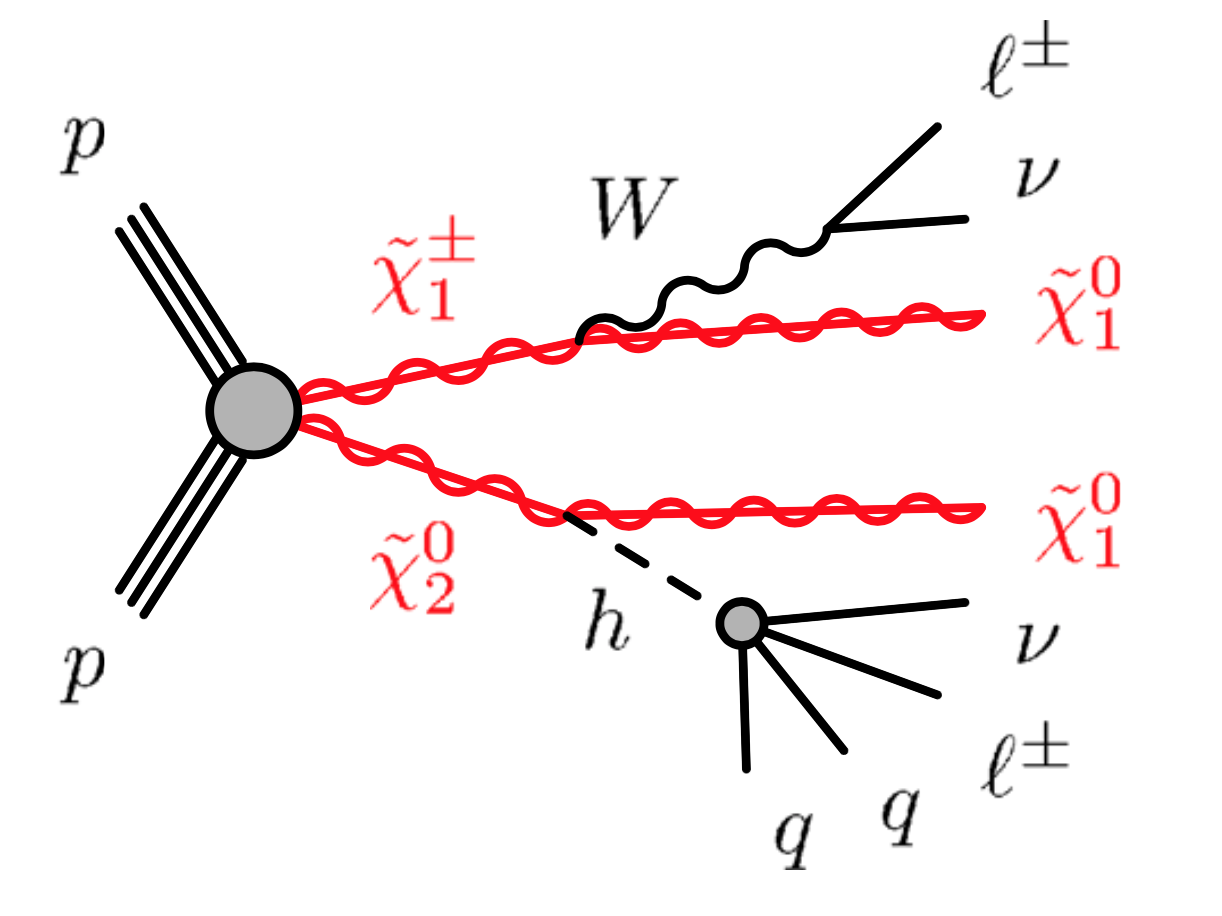
\includegraphics[width=0.3\textwidth]{data/photo/theory/signal_feynman.png}
\end{figure}
\end{frame}

\begin{frame}{Our Signal Scenario : Sensitive Region}
\begin{itemize}
\item If the mass difference ($m_{\tilde{\chi}_1^\pm , \tilde{\chi}_2^0} - m_{\tilde{\chi}_1^0}$) is slightly larger than the Higgs mass, it is called the compressed region.
\item In the compressed region, one of the lepton may have low energy, due to the low momentum of the Higgs boson, and hence it may not be detected.
\item In this case, there may be originally 3 leptons, but only 2 leptons are detected.
\item This allows more decay modes for Higgs boson, which produce two leptons. (For example, $h \rightarrow ZZ$)
\item Hence, the signal will be more sensitive in the compressed region.
\end{itemize}
\end{frame}

\end{document}
